\documentclass{article}
\usepackage{tikz}
\usetikzlibrary{fit}

\title{The simple math of mempool hierarchies}

\author{Tobias Heindel}

\usepackage{hyperref,amsmath,amssymb,amsthm}
\newtheorem{definition}{Definition}
\usepackage{newunicodechar}
\newunicodechar{∈}{\in}
\newunicodechar{ℕ}{\mathbb{N}}

\begin{document}

\maketitle
\begin{abstract}
  This document provides the generic mathematical calculations.
\end{abstract}

\section{Things to keep in mind: conventions}
\label{sec:conventions}

\begin{description}
\item[Pool]
  While our terminology is inspired by mempools
  as found in block chains of the first generation(s),
  most notably Bitcoin and Ethereum,
  we shall simply speak of \emph{pools};
  a related work are \emph{dark pools},
  and comparison of feature sets with the latter may be of independent interest.
  However,
  we do not want to impose any specific restrictions on the
  pool contents.
\item[Pool elements]
  Often we simply speak of \emph{elements} of pools,
  which makes sense as the latter are ``replicated multi-sets''—at
  least conceptually.
  Elements are ``opaque'',
  very much like an \href{https://en.wikipedia.org/wiki/Urelement}{urelement};
  in technical terms,
  they are just blobs of binary data.
\item[Elements size]
  Each element $e$ has a fixed size $|e|∈ℕ$.
\item[Inflow]
  We shall speak of \emph{inflow} of elements.
\item[Solution]
  We abstract away the specific type of solving,
  but consider solutions of a set of elements,
  such that the solution of a set of elements is bounded by
  a polynomial over sum of the sizes in a set of events.
\end{description}

\section{The arity of the tree: $\boldsymbol d$}%
\label{sec:tree-arity}

We fix~$d ∈ ℕ \setminus \{ 0, 1 \}$,
the arity of the tree.
Given the height~$h\in ℕ$, 
the \emph{root pool} has size~$d^h$;
recall that the height is the length of the longest path in the tree
where path length is counted in the number of edges.
If the height is zero,
we have the degenerate case of
a tree that is just the root node.

\section{Delay (over-)approximations}%
\label{sec:delay-approximations}

First there are two types of delays, namely
\emph{consensus delay} and the \emph{solving delay}.

\subsection{Consensus delay}
\label{sec:consesnus-delay}

Consensus introduces additional delay,
due to the distributed setting.
The reason is that pool operators have to agree upon
the canonical contents of the next batch
(to be used as input to the next round of solving).
The consensus delay is relative to a specific pool in the tree.
We are mainly interested in the average delay
that (correct) operators can measure.\footnote{%
  Definition~\ref{def:consensus-delay-avg}
  can obviously be adapted to 
}% ᚦ: let us see what we really need
\begin{definition}[Consensus Delay, in average]
  \label{def:consensus-delay-avg}
  Consensus delay in average,
  is the average time span
  between the arrival of a last pool element
  and the consensus being decided,
  among correct operators.
\end{definition}

We consider the perfectly decentralized scenario,
where each operator has the same voting power.
We assume that the consensus algorithm used has a
constant minimum number of \emph{message delays}.

The best case scenario in a leader based protocol
is that the leader is roughly in the middle of the relevant quorum.


The worst case concerns
the leader being at maximal distance in sum
to the remainder of the quorum.
\begin{center}
  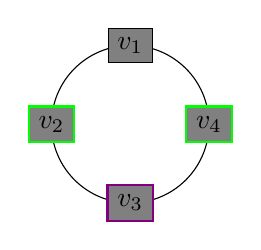
\begin{tikzpicture}
    \foreach \x in {1,...,4}{
      \coordinate(c\x) at (\x*90:1);
    }
    \draw (0,0) circle (1);
    \foreach \x in {1,...,4}{
      \node[fill=gray,draw] (v\x) at (c\x) {$v_{\x}$};
    }
    \begin{scope}[double]
      \foreach \x in {2,4}
      \node[draw,green,thick,fit=(v\x),rectangle,inner sep=0pt] {};
      \node[draw,violet,thick,fit=(v3),rectangle,inner sep=0pt] {};
    \end{scope}
\end{tikzpicture}
\end{center}
In the worst case(s),
the leader has to communicate with a node
on the opposite side of the circle.
\begin{center}
  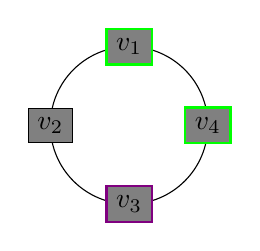
\begin{tikzpicture}
    \foreach \x in {1,...,4}{
      \coordinate(c\x) at (\x*90:1);
    }
    \draw (0,0) circle (1);
    \foreach \x in {1,...,4}{
      \node[fill=gray,draw] (v\x) at (c\x) {$v_{\x}$};
    }
    \begin{scope}[double]
      \foreach \x in {1,4}
      \node[draw,green,thick,fit=(v\x),rectangle,inner sep=0pt] {};
      \node[draw,violet,thick,fit=(v3),rectangle,inner sep=0pt] {};
    \end{scope}
\end{tikzpicture}
\end{center}
For the case on the line (or if the diameter is huge),
the situation is slightly different.

\begin{center}
  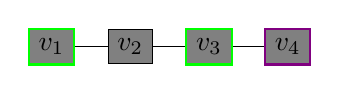
\begin{tikzpicture}
    \foreach \x in {1,...,4}{
      \coordinate(c\x) at (\x,0);
    }
    \draw (c1) -- (c4);
    \foreach \x in {1,...,4}{
      \node[fill=gray,draw] (v\x) at (c\x) {$v_{\x}$};
    }
    \begin{scope}[double]
      \foreach \x in {1,3}
      \node[draw,green,thick,fit=(v\x),rectangle,inner sep=0pt] {};
      \node[draw,violet,thick,fit=(v4),rectangle,inner sep=0pt] {};
    \end{scope}
\end{tikzpicture}
\end{center}
Here we have a factor three between best and worst case.

\begin{center}
  \large do some calculations
\end{center}

\end{document}

%%% Local Variables:
%%% mode: LaTeX
%%% TeX-master: t
%%% End:
